\documentclass[handout]{beamer}

\usepackage{graphicx, subfigure}
\usepackage{amsmath}


% \usepackage{beamerthemesplit} // Activate for custom appearance


\title{\color{magenta} Introduction to Knock-off Filters}
\subtitle{\color{blue}``Controlling False Discovery Rates via Knock-offs "\\ Authors: Rina Barber and Emmanuel Candes }
\author{ Nandana Sengupta}
\date{\color{olive}\today}

\begin{document}

\frame{\titlepage}

\frame{
\frametitle{Introduction}
\color{magenta}
"All models are wrong, but some models are useful" -- George Box 
\vspace{2em}
\color{olive}
\begin{itemize}
\item<2-> Consider the simple linear regession model:
 \color{olive}$$y = X \beta + \varepsilon; \qquad y \in \mathbb{R}^n, \quad X \in \mathbb{R}^{n \times p}, \quad \varepsilon \sim N(0,\sigma^2) $$
$$\Rightarrow  \hat{\beta}_{ols} = \underset{\beta}{\mbox{argmin}} \left(y - X\beta\right)' \left(y - X\beta\right) $$
\begin{itemize}
\item<3-> {\color{magenta}Large number of $X$}: low bias but larger variance
\item<4-> {\color{magenta}Small number of $X$}: higher bias but small variance
\item<5-> {\color{magenta}Ideal}: Small set of $X$ truly associated with $y$
\end{itemize}
\vspace{2em}
\item<7-> Motivating example from genetics:
\begin{itemize}
\item<8-> {\color{magenta} $y$}: phenotype (observable traits eg: eye color, height)
\item<9-> {\color{magenta} $X$}: genes
\end{itemize}



\end{itemize}
}




\frame{
\frametitle{Introduction}
\color{magenta}
"All models are wrong, but some models are useful" -- George Box 
\vspace{2em}
\color{olive}
\begin{itemize}
\item Consider the simple linear regession model:
 \color{olive}$$y = X \beta + \varepsilon; \qquad y \in \mathbb{R}^n, \quad X \in \mathbb{R}^{n \times p}, \quad \varepsilon \sim N(0,\sigma^2) $$
$$\Rightarrow  \hat{\beta}_{ols} = \underset{\beta}{\mbox{argmin}} \left(y - X\beta\right)' \left(y - X\beta\right) $$
\begin{itemize}
\item {\color{magenta}Large number of $X$}: low bias but larger variance
\item {\color{magenta}Small number of $X$}: higher bias but small variance
\item {\color{red}\textbf{Ideal: Small set of $X$ truly associated with $y$ $ \mathbf{\Longleftarrow} $}}
\end{itemize}
\vspace{2em}
\item \color{black}Motivating example from genetics:
\begin{itemize}
\item {\color{magenta} $y$}: phenotype (observable traits eg: eye color, height)
\item {\color{magenta} $X$}: genes
\end{itemize}



\end{itemize}
}




\frame{
\frametitle{Preliminary Concept 1: Variable Selection Techniques}
\begin{center}{\color{magenta}``Selecting a Small Subset of Variables"} \end{center}
\begin{itemize}
\item<2->   Forward Stepwise Regression
\item<3-> Backward Stepwise Regression
\item<4-> \color{magenta}$\Rightarrow$\textbf{LASSO} 
\item<5-> {\color{olive} \begin{center}
 $ \hat{\beta}_{\lambda} = \underset{\beta}{\mbox{argmin}} \left(y - X\beta\right)' \left(y - X\beta\right) + \lambda \sum_{j=1}^{p} |\beta_j|  $ \end{center}} 

\item<6->  \begin{center}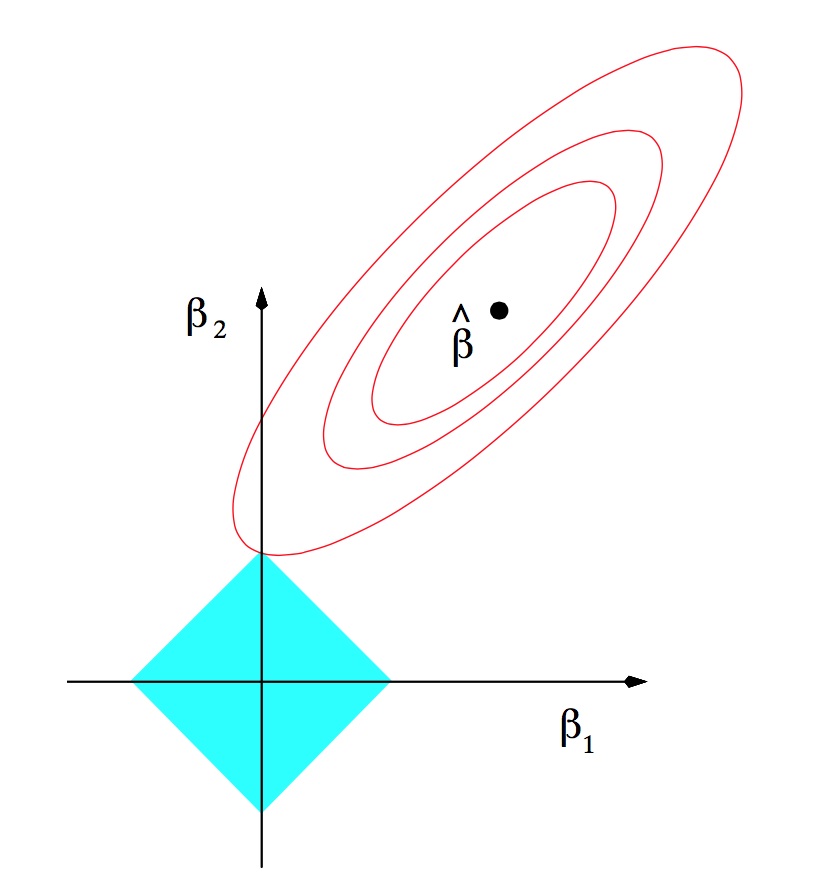
\includegraphics[width=.5\linewidth]{lasso} \end{center}

\end{itemize}
}



\frame{
\frametitle{Preliminary Concept 1: Variable Selection Techniques}
\begin{center}{\color{magenta}``Selecting a Small Subset of Variables"} \end{center}
\begin{center}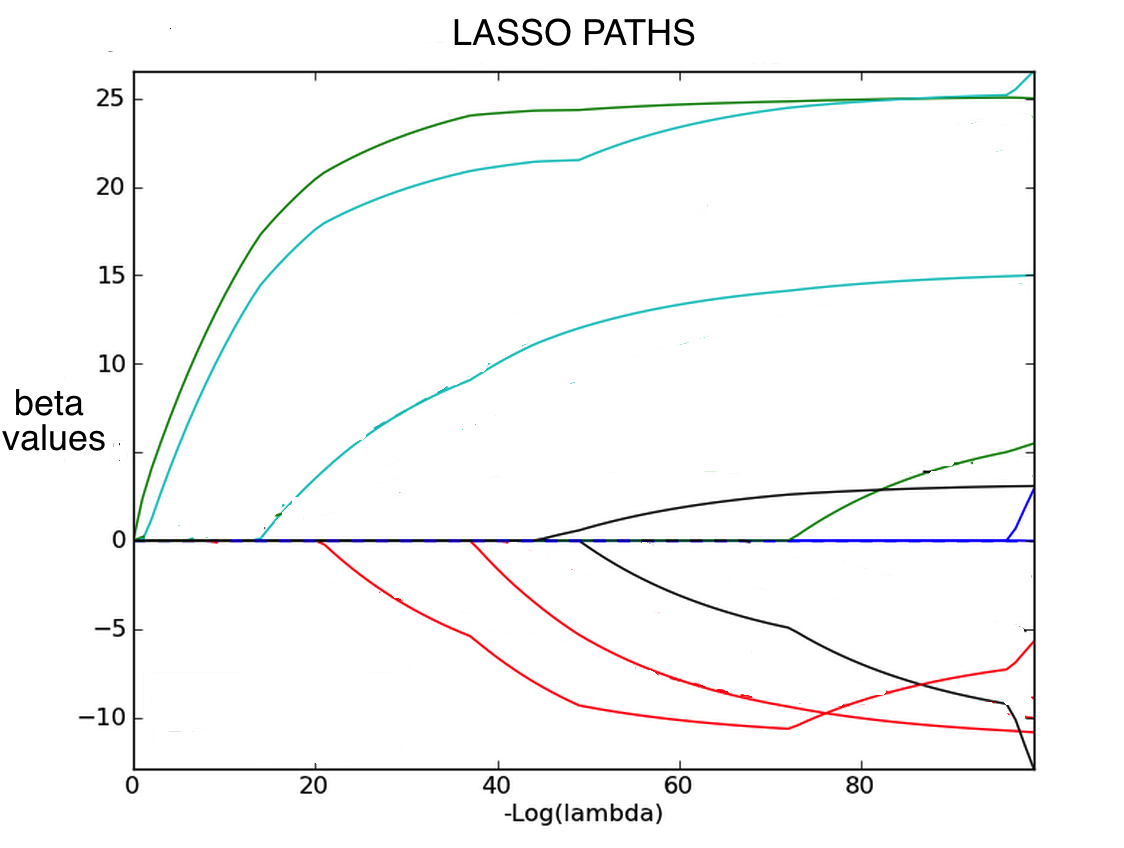
\includegraphics[width=.75\linewidth]{paths} \end{center}


}




\frame{
\frametitle{Preliminary Concept 2: False Discovery Rate}
\begin{center}{\color{magenta}``Selecting Variables {\color{red}\textbf{truly associated}} with y. "} \end{center}
\begin{itemize}
\item<2-> Null hypothesis   $\color{olive} \mathcal{H}_0:  \beta_j = 0$
\item<3-> Set of selected covariates: $\color{olive} \mathcal{S}$ 
\item<4->\begin{center} 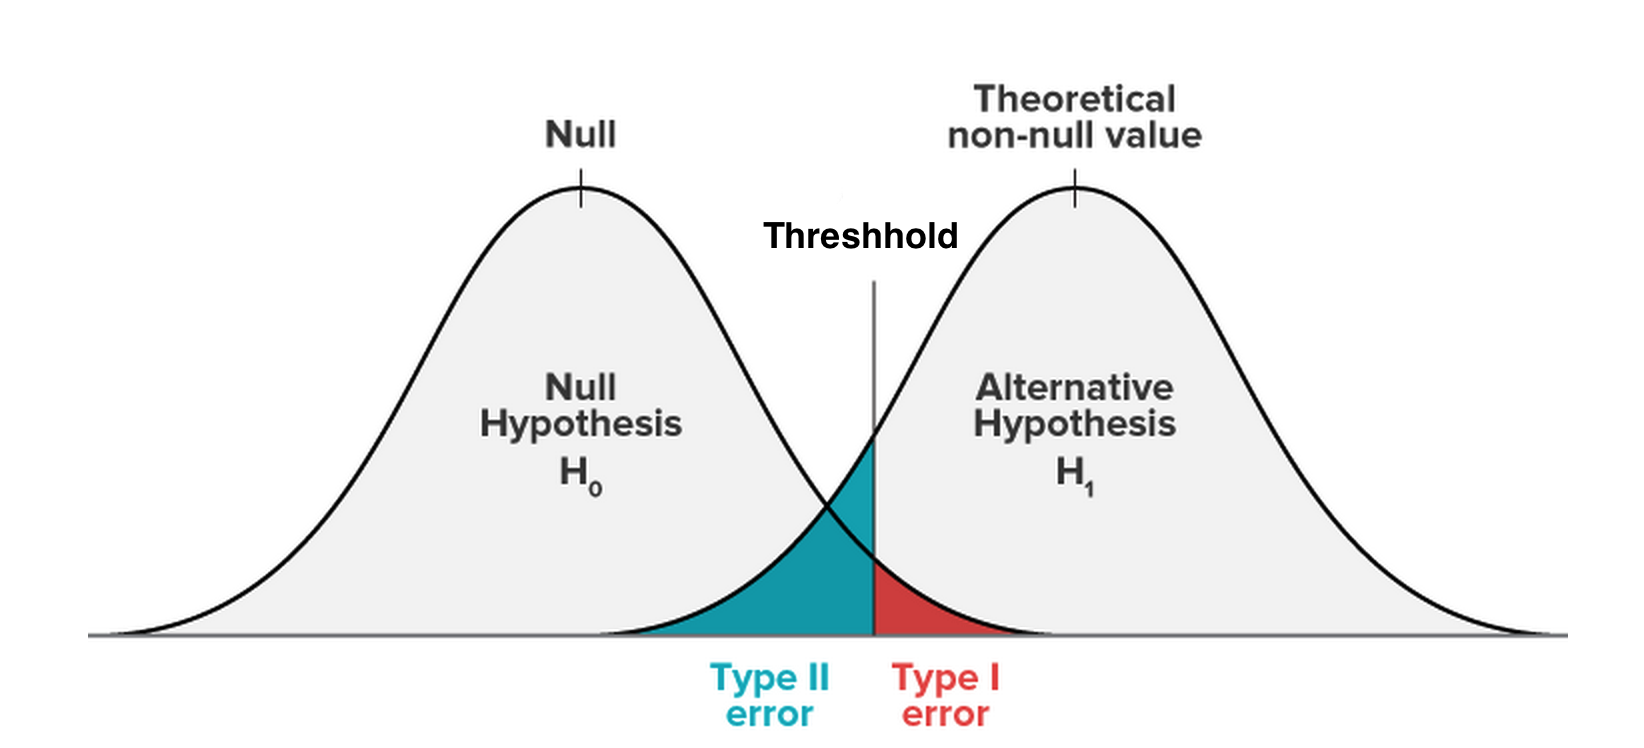
\includegraphics[width = 0.75 \textwidth]{errors} \end{center}
\item<5-> Want to control the proportion of \color{magenta} Type I error
\item<6-> \begin{center} 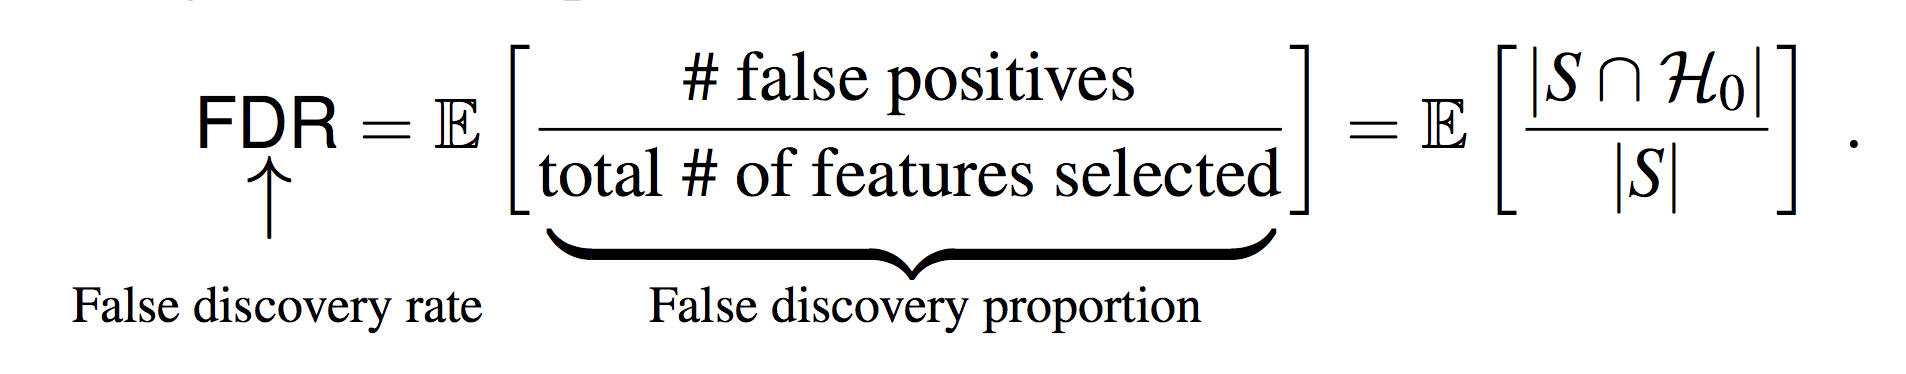
\includegraphics[width = 0.75 \textwidth]{fdr} \end{center}
\item<7-> Work by Benjamini-Hochberg (1995, 2000)
\end{itemize}
}




\frame{
\frametitle{Knock-off Filters: Algorithm}

\begin{itemize}
\item<2-> \color{magenta} Step 1: Construct Knock-offs $\tilde{X}$ such that
\begin{itemize}

\item<3-> {\color{olive} Correlation Structure:} $\tilde{X}'\tilde{X} = X'X = \Sigma $
\item<4->{\color{olive} Correlation Structure:} $X'\tilde{X}=  \Sigma - diag(s)$
\item<5->{\color{olive} How? }$\tilde{X} = X(I- \Sigma^{-1} diag(s) )+ \tilde{U} C$
\item<6->{\color{olive}Augmented Matrix:} $[X \quad \tilde{X}]$
\end{itemize}
\item<7-> \color{magenta}  Step 2: Compute Lasso with Augmented Matrix
 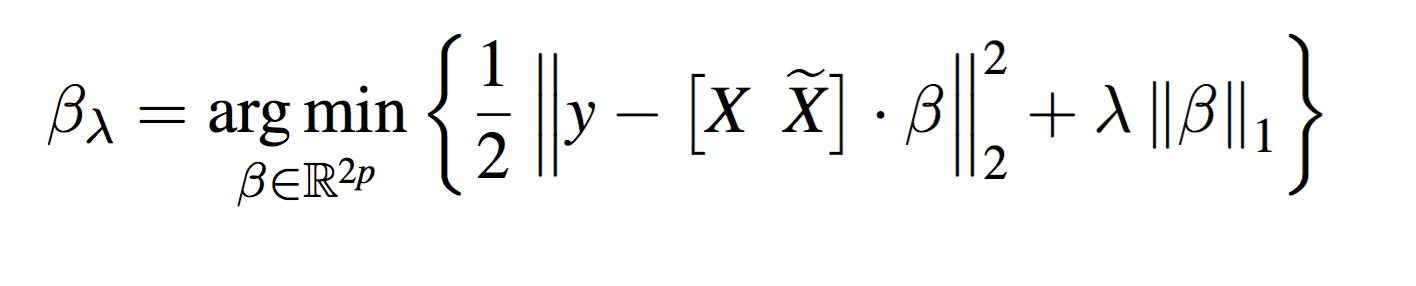
\includegraphics[width = 0.75 \textwidth]{auglas} 
\item<8-> \color{magenta} Step 3: For each pair of knock-off and original variables, calculate 

\item<9-> 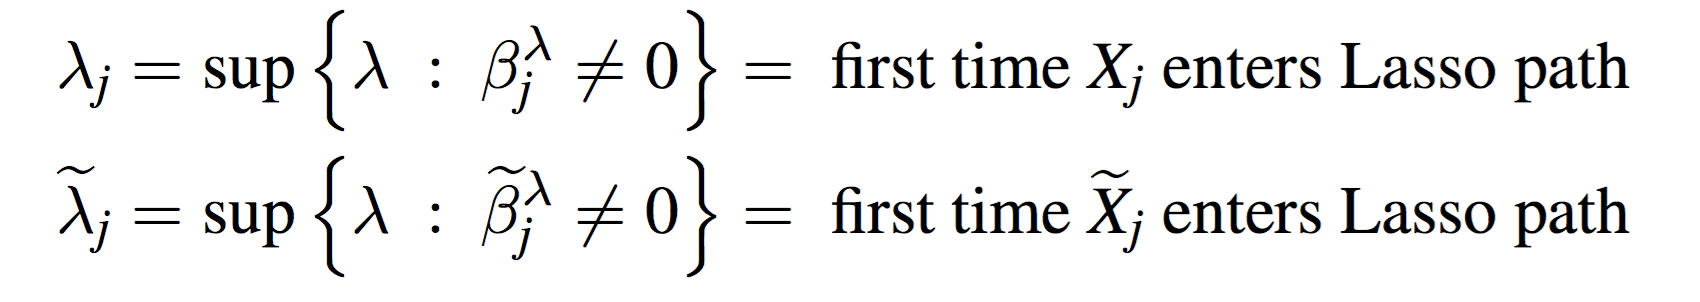
\includegraphics[width = 0.75 \textwidth]{auglambda} \\
 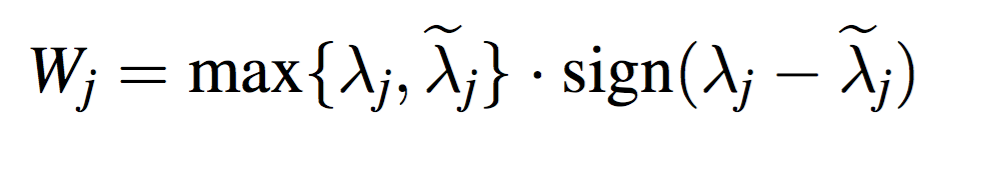
\includegraphics[width = 0.45 \textwidth]{auglambda1} 

\end{itemize}
}





\frame{
\frametitle{Knock-off Filters: Algorithm}
\begin{itemize}
\item<2->\color{magenta} Step 4: For each $\lambda$ value calculate
\item<3-> 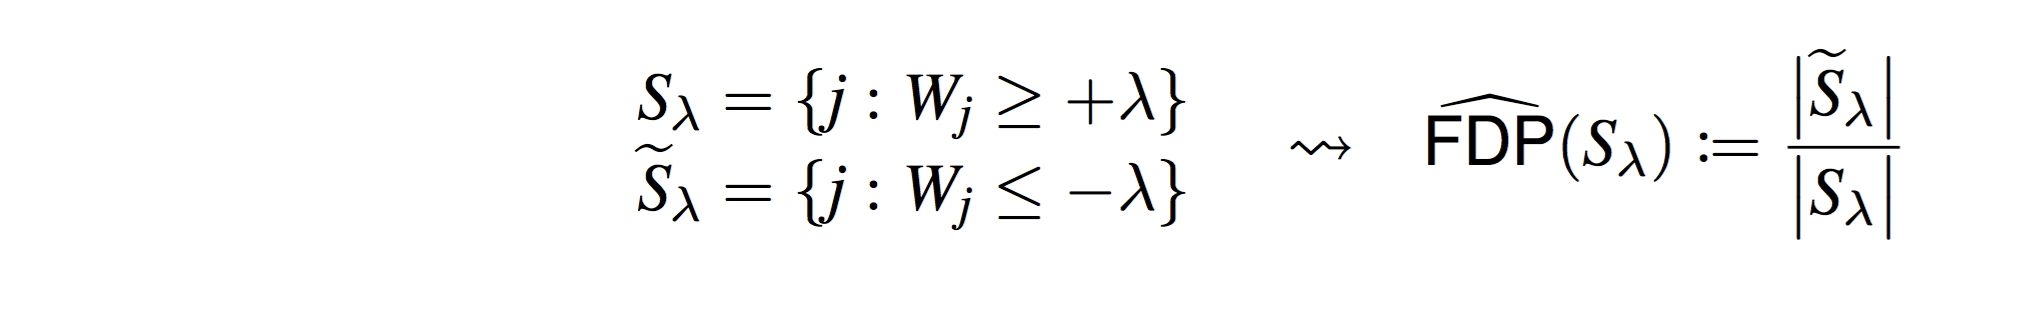
\includegraphics[width =  \textwidth]{fdp}  

\item<4-> \color{magenta} Step 5: Choose threshold level $q$
\item<5-> \color{magenta} Step 6: Select the variables based on
\item<6->
$$\Lambda = min \{ \lambda: \widehat{FDP}(S_\lambda) \leq q \} $$
$$ S_{\Lambda} = \{j : W_j \geq \Lambda \} $$
\item<7-> \color{magenta} Knock-off+ filter: 
\item<8->\begin{center}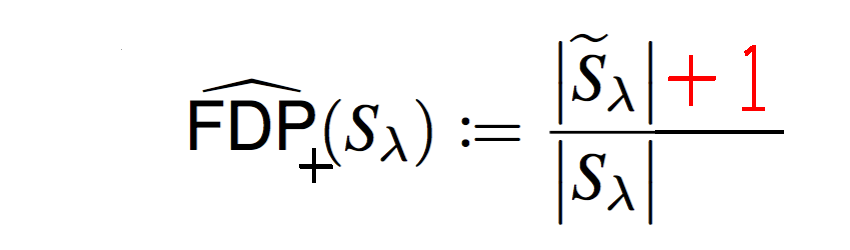
\includegraphics[width = 0.35 \textwidth]{fdp+} \end{center}
\end{itemize}
}



\frame{
\frametitle{Knock-off Filters: Intuition}
 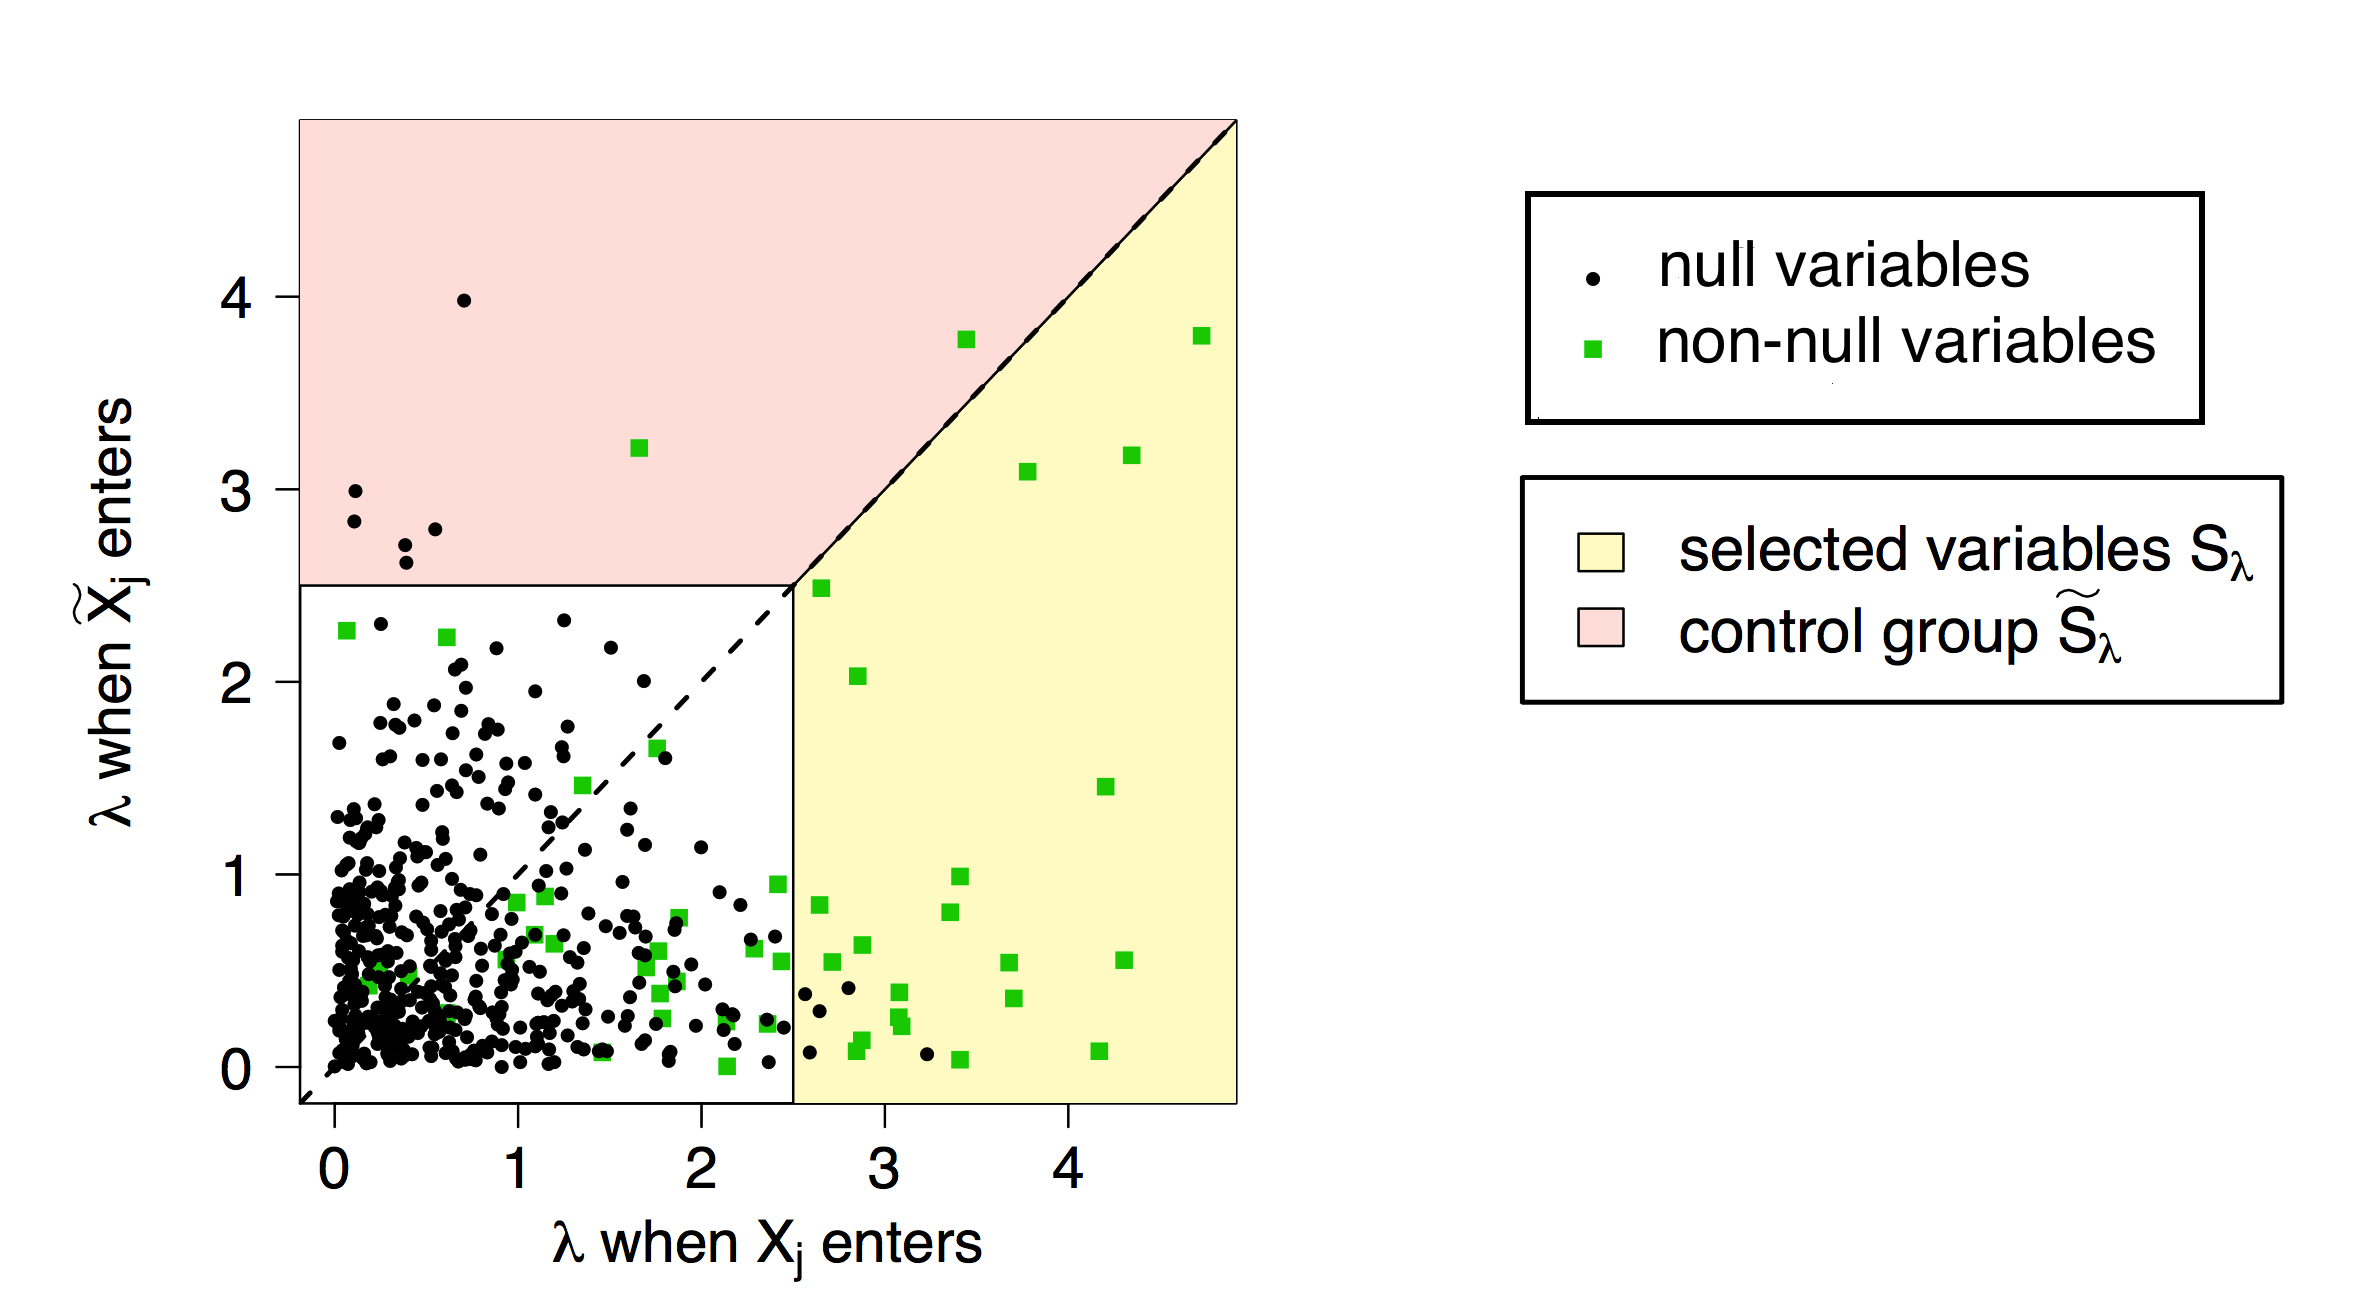
\includegraphics[width = 1.05 \textwidth]{slambdafig} 

}





\frame{
\frametitle{Rest of the paper}
\begin{itemize} 

\item<2-> \color{magenta}Theoretical Guarantees
\begin{itemize}
\item<3->  {\color{olive}Theorem 1:} $\mathbb{E}[mFDP(S_{\Lambda})] \leq q ; \quad mFDP(S) = \frac{|S \cap \mathcal{H}_0| }{|S|+q^{-1} }  $ 
\item<4->  { \color{olive}Theorem 2:} $\mathbb{E}[FDP(S_{\Lambda_+})] \leq q $
\end{itemize} 
\item<5-> \color{magenta} Simulation Results
\begin{itemize}
\item<6-> Compare knock-off, knock-off+ \& Benjamini-Hochberg 
\item<7-> All three techniques lead to FDR below threshold $q$
\item<8-> knock-off, knock-off+ perform better in terms of power 
\item<9-> Power: \color{olive}$1- Pr(\mbox{Type II Error})$
\end{itemize}

\item<9-> \color{magenta} Empirical Application
\begin{itemize}
\item<10->  model drug resistance of HIV-1 ({\color{olive}$y$}) on genetic mutations ({\color{olive}$X$})
\end{itemize}


\end{itemize}
}




\frame{
\frametitle{Going Further: Issues and Possible Applications}
\begin{itemize}
\item<2-> \color{magenta}Paper makes very few assumptions:
\begin{itemize}
\item<3->  Don't need to know $\sigma^2$
\item<4-> Don't need any information on $\beta$
\end{itemize}
\item<5-> \color{magenta}But those that it makes may be critical:
\begin{itemize}
\item<6-> Full rank $X'X = \Sigma $  
\item<7-> $n > p$
\item<8-> Most practical applications of LASSO not suitable
\item<9-> Ongoing work on these aspects
\end{itemize}
\item<10-> {\color{magenta} General issue with LASSO:} Confidence interval estimation
\vspace{2em}
\item<11-> \color{olive} Possible Applications:
\begin{itemize}
\item<12-> Useful when we don't have any model of the response.
\item<13-> Worthwhile to think about $2-step$ methods (?)
\item<14-> Effect of a particular covariate on response but not sure about others covariates (?)
\end{itemize}

\end{itemize}
}


\frame{
\begin{center}
Thanks! 
\end{center}
}


\end{document}

